  \documentclass{beamer}

% Used packages
\usepackage[utf8]{inputenc}
\usepackage[spanish]{babel}
\usepackage{amssymb, amsmath, amsthm, amsfonts, esint, mathtools}
\usepackage{hyperref}
\usepackage{graphicx}
\usepackage{subfig}




% There are many different themes available for Beamer. A comprehensive
% list with examples is given here:
% http://deic.uab.es/~iblanes/beamer_gallery/index_by_theme.html
% You can uncomment the themes below if you would like to use a different
% one:
%\usetheme{AnnArbor}
\usetheme{Antibes}
%\usetheme{Bergen}
%\usetheme{Berkeley}
%\usetheme{Berlin}
%\usetheme{Boadilla}
%\usetheme{boxes}
%\usetheme{CambridgeUS}
%\usetheme{Copenhagen}
%\usetheme{Darmstadt}
%\usetheme{default}
%\usetheme{Frankfurt}
%\usetheme{Goettingen}
%\usetheme{Hannover}
%\usetheme{Ilmenau}
%\usetheme{JuanLesPins}
%\usetheme{Luebeck}
%\usetheme{Madrid}
%\usetheme{Malmoe}
%\usetheme{Marburg}
%\usetheme{Montpellier}
%\usetheme{PaloAlto}
%\usetheme{Pittsburgh}
%\usetheme{Rochester}
%\usetheme{Singapore}
%\usetheme{Szeged}
%\usetheme{Warsaw}
%\justifying
\renewcommand{\raggedright}{\leftskip=0pt \rightskip=0pt plus 0cm} 

\title{Avance de Proyecto}

% A subtitle is optional and this may be deleted
\subtitle{Identificación facial con pocas muestras por clase}

\author{Martín Villanueva\inst{1}}
% - Give the names in the same order as the appear in the paper.
% - Use the \inst{?} command only if the authors have different
%   affiliation.

\institute[Universidad Técnica Federico Santa María] % (optional, but mostly needed)
{
  \inst{1}%
  Departamento de Informática\\
  Universidad Técnica Federico Santa María}
% - Use the \inst command only if there are several affiliations.
% - Keep it simple, no one is interested in your street address.

\date{Máquinas de Aprendizaje, 2015}
% - Either use conference name or its abbreviation.
% - Not really informative to the audience, more for people (including
%   yourself) who are reading the slides online

%\subject{Theoretical Computer Science}
% This is only inserted into the PDF information catalog. Can be left
% out.

% If you have a file called "university-logo-filename.xxx", where xxx
% is a graphic format that can be processed by latex or pdflatex,
% resp., then you can add a logo as follows:

% \pgfdeclareimage[height=0.5cm]{university-logo}{university-logo-filename}
% \logo{\pgfuseimage{university-logo}}

% Delete this, if you do not want the table of contents to pop up at
% the beginning of each subsection:
\AtBeginSection[]
{
  \begin{frame}<beamer>{Outline}
    \tableofcontents[currentsection,currentsubsection]
  \end{frame}
}

% Let's get started
\begin{document}

\begin{frame}
  \titlepage
\end{frame}



\begin{frame}{Outline}
  \tableofcontents
  % You might wish to add the option [pausesections]
\end{frame}




% Section and subsections will appear in the presentation overview
% and table of contents.
\section{El Problema}
\subsection{Identificación facial}

\begin{frame}{Definición del Problema}

El problema tratado consiste en, dadas una \textit{pocas} muestras de imagenes faciales de distintos individuos, generar un algoritmo que permita identificar correctamente a cada individuo, dada una imagen distinta a las anteriores. Más formalmente:

\begin{itemize}
 \item Se define $S_{tr} =  \{\mathbf{s}_1 , \ldots, \mathbf{s}_M \}$ como el conjunto de entrenamiento con imágenes faciales de $K$ individuos. 
 \item El problema de \textbf{identificación} es, dada una imagen de \textit{test} $\mathbf{p}$, determinar cuál de las $K$ clases del conjunto de entrenamiento $S_{tr}$ corresponde.
 \item Se restringe el problema a casos donde cada clase posee pocas muestras en $S_{tr}$, lo cual es una situación bastante realista.
\end{itemize}
\end{frame}


\subsection{Datasets}


\begin{frame}{Datasets}
Los datasets a ocupar corresponden a \href{http://cswww.essex.ac.uk/mv/allfaces/faces94.html}{Faces94} y
\href{http://cswww.essex.ac.uk/mv/allfaces/faces95.html}{Faces95}. Los cuales tiene las siguientes características 
respectivamente:
\begin{itemize}
	\item \textbf{Faces94}: $153$ individuos, $20$ imágenes por individuo, resolución $200\times 180$, hombres y mujeres, fondo fijo, poca variación en escalamiento, poca variación de posición de la imagen y condiciones de iluminación, y considerables variaciones en expresiones faciales.
	\item \textbf{Faces95}: $72$ individuos, $20$ imágenes por individuo, resolución $200\times 180$, hombres y mujeres, fondo con sombra, considerable variación en escalamiento, poca variación en posición de imagen, iluminación variable, y variaciones considerable en expresiones faciales.
\end{itemize}
\end{frame}

\begin{frame}{Faces94}

\begin{figure}
\begin{tabular}{ccc}
\subfloat{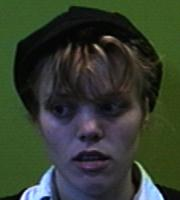
\includegraphics[width = .9in]{faces94_1}} &
\subfloat{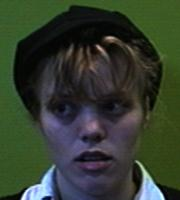
\includegraphics[width = .9in]{faces94_2}} &
\subfloat{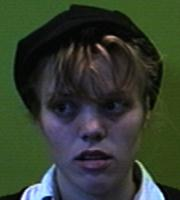
\includegraphics[width = .9in]{faces94_3}}\\
\subfloat{
\includegraphics[width = .9in]{faces94_4}} &
\subfloat{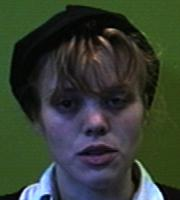
\includegraphics[width = .9in]{faces94_5}} &
\subfloat{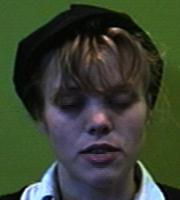
\includegraphics[width = .9in]{faces94_6}}
\end{tabular}
\caption{Imágenes características de un individuo en Faces94}
\end{figure}
	
\end{frame}

\begin{frame}{Faces95}
 
\begin{figure}
\begin{tabular}{ccc}
\subfloat{
\includegraphics[width = .9in]{faces95_1}} &
\subfloat{
\includegraphics[width = .9in]{faces95_2}} &
\subfloat{
\includegraphics[width = .9in]{faces95_3}}\\
\subfloat{
\includegraphics[width = .9in]{faces95_4}} &
\subfloat{
\includegraphics[width = .9in]{faces95_5}} &
\subfloat{
\includegraphics[width = .9in]{faces95_6}}
\end{tabular}
\caption{Imágenes características de un individuo en Faces95}
\end{figure}

\end{frame}


\begin{frame}{Otras consideraciones}
 Para emular las reestriciones del problema, se sigue la siguiente metodología
 \begin{itemize}
 	\item Para cada uno \textbf{Faces94} y \textbf{Faces95} se generan 20 training y testing sets respectivos.
 	\item Cada training set se genera tomando $3-5$ muestras aleatoreas por cada individuo, dejando el resto de las $15-17$ imágenes restantes en el testing set. 
 	\item Luego, para cada dataset (\textbf{Faces94} o \textbf{Faces95}) hay en total $60$ sets de training y testing
 	respectivos.
 	\item La presentación de resultados, se realiza con Errorbars (t-student $95\%$ de confianza) del error rate sobre los 20 datasets respectivos. 
 \end{itemize}
\end{frame}

\section{Propuestas de solución}

\subsection{Linear Discriminant Analysis}
\begin{frame}{LDA}
\begin{itemize}
	\item La implementación ocupada corresponde la de Scikit-Learn. Para cada una de las clases (personas) genera un función discriminante lineal $\delta_k$, que permite diferenciar a cada una de las clases. 
	\item Supuestos Fuertes: 1) La probabilidad multivariada de las características $P(x_m | y=k)$ se distribuye normal, y  2) La matriz de covarianza para cada una de las clases es igual.
	\item Como LDA es un modelo generativo (sin hiperparámetros), no es necesario realizar cross-validation para el modelo. Permite ahorar gran tiempo de computación.
\end{itemize}
\end{frame}

\begin{frame}{LDA: Resultados en Faces94}
\begin{figure}[htpb!]
\centering
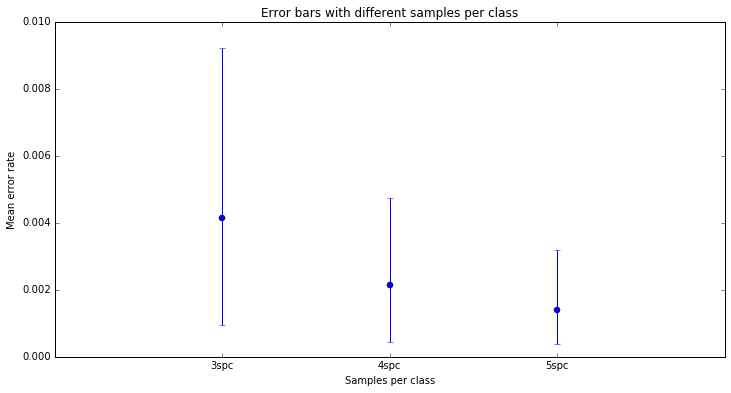
\includegraphics[width=10cm]{lda_res94}
\caption{Resultados obtenidos con LDA en \textbf{Faces94}}
\end{figure}
\end{frame}

\begin{frame}{LDA: Resultados en Faces95}
\begin{figure}[htpb!]
\centering
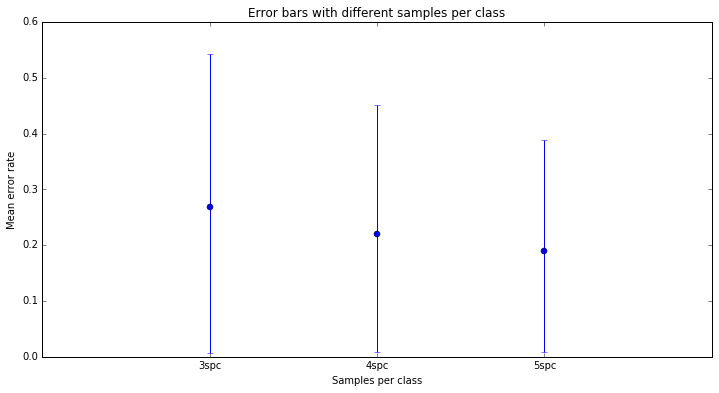
\includegraphics[width=10cm]{lda_res95}
\caption{Resultados obtenidos con LDA en \textbf{Faces95}}
\end{figure}
\end{frame}

\subsection{Multi-class SVM}

\begin{frame}{Multi-class SVM}
\begin{itemize}
	\item Support Vector Machines (SVM) es un método de clasificación binario (adaptable a problemas de múltiples clases), que encuentra la frontera de decisión lineal óptima (hiperplano óptimo) separadora de las clases.
	\item Implementación y entrenamiento de multiclass SVM's con kernels tanto lineales como RBF. La implementación de Scikit-Learn advierte: “SVC implement one-against-one” approach (Knerr et al., 1990) for multi- class classification".
	\item Se utilizan $\nu$-SMV's, debido a que facilita la configuración del parámetro de holgura $\nu \in (0,1]$, y a su interpretación.
	\item Selección de hiperparámetros $\nu$ y $\gamma$ (en kernels rbf) se realiza stratified cross-validation. Para que esto tenga sentido, el número de folds debe ser igual al número de muestras por clase.
\end{itemize}
\end{frame}

\begin{frame}{Reducción de dimensionalidad}
\begin{itemize}
	\item \textbf{Problema:} Las dimensiones de las imágenes (200x180=36000) corresponden al total de features de cada foto. Esto hace necesario ocupar reducción de dimensionalidad para tomar las características realmente importantes (aquellas que permiten diferencias entre las clases) y mejorar los tiempos de entrenamientos y eficiencia.
	\item Como técnica de reducción de dimensionalidad, se ha decidido ocupar LDA, representación tambien conocida como Fisher Faces (reducción de dimensionalidad supervisada).
	\item \textbf{Idea:} Proyectar la data en espacio donde se maximice la inter-class variance y minimice la intra-class variance. 
\end{itemize}
\end{frame}


\begin{frame}{Reducción de dimensionalidad (2)}
\begin{figure}[htpb!]
\centering
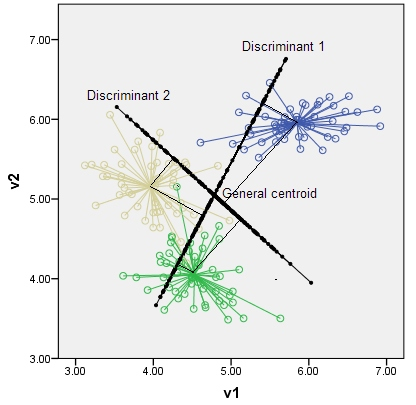
\includegraphics[width=4cm]{fisherfaces}
\caption{LDA como reducción de dimensionalidad}
\end{figure}

\begin{itemize}
	\item El número de máximo de discriminantes es $\min(\text{dim},K-1)$, por lo tanto en un problema con muchas más dimensiones (features) que clases, la reducción de dimensionalidad es considerablemente. 
\end{itemize}
\end{frame}

\begin{frame}{Resultados linear SVM Faces94}
\begin{figure}[htpb!]
\centering
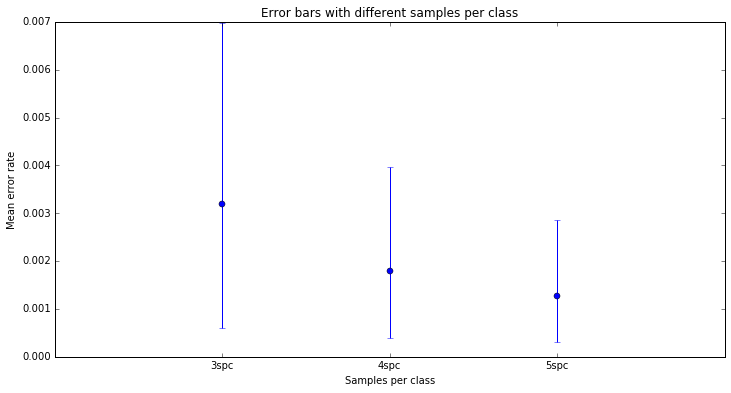
\includegraphics[width=10cm]{lsvm_res94}
\caption{Resultados obtenidos con linear SVM en \textbf{Faces94}}
\end{figure}
\end{frame}

\begin{frame}{Resultados linear SVM Faces94 (2)}
\begin{figure}[htpb!]
\centering
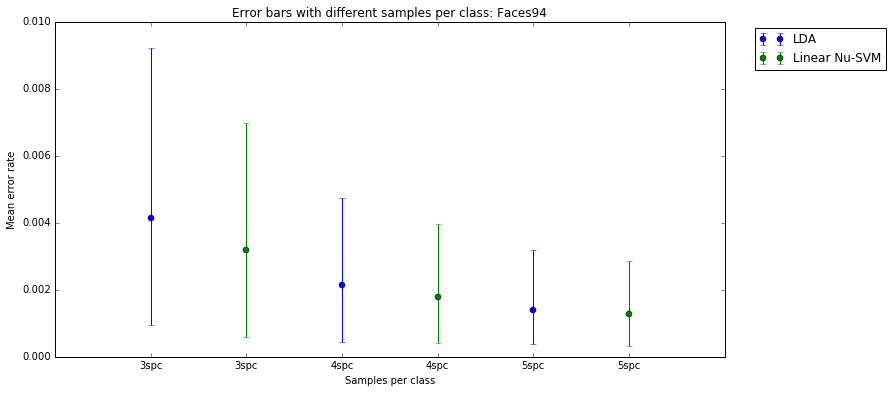
\includegraphics[width=10cm]{lsvm_rescomp94}
\caption{Comparación de resultados obtenidos con linear SVM en \textbf{Faces94}}
\end{figure}
\end{frame}

\begin{frame}{Resultados linear SVM Faces95}
\begin{figure}[htpb!]
\centering
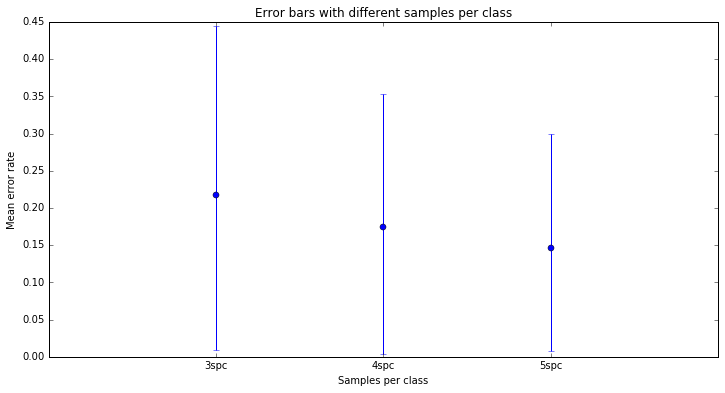
\includegraphics[width=10cm]{lsvm_res95}
\caption{Resultados obtenidos con linear SVM en \textbf{Faces95}}
\end{figure}
\end{frame}

\begin{frame}{Resultados linear SVM Faces95 (2)}
\begin{figure}[htpb!]
\centering
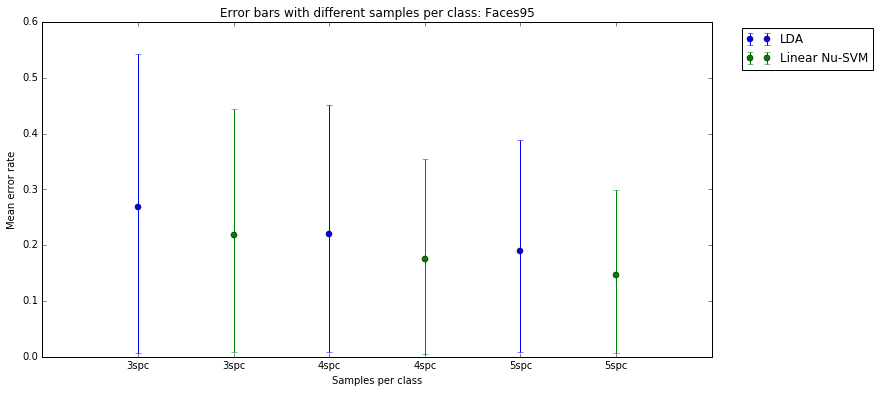
\includegraphics[width=10cm]{lsvm_rescomp95}
\caption{Comparación de resultados obtenidos con linear SVM en \textbf{Faces95}}
\end{figure}
\end{frame}

\begin{frame}{Resultados RBF SVM Faces94}
\begin{figure}[htpb!]
\centering
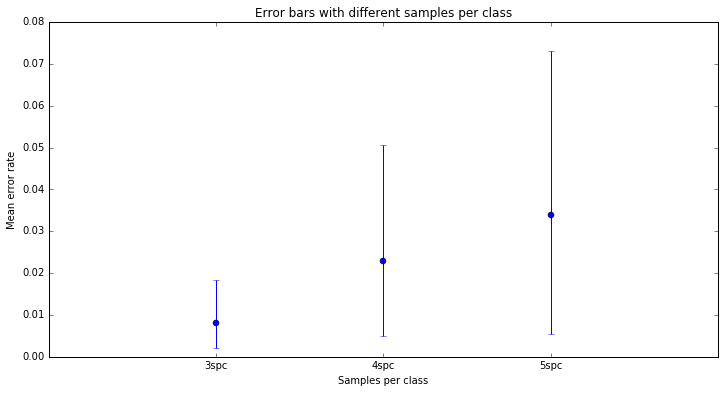
\includegraphics[width=10cm]{ksvm_res94}
\caption{Resultados obtenidos con RBF SVM en \textbf{Faces94}}
\end{figure}
\end{frame}

\begin{frame}{Resultados RBF SVM Faces94 (2)}
\begin{figure}[htpb!]
\centering
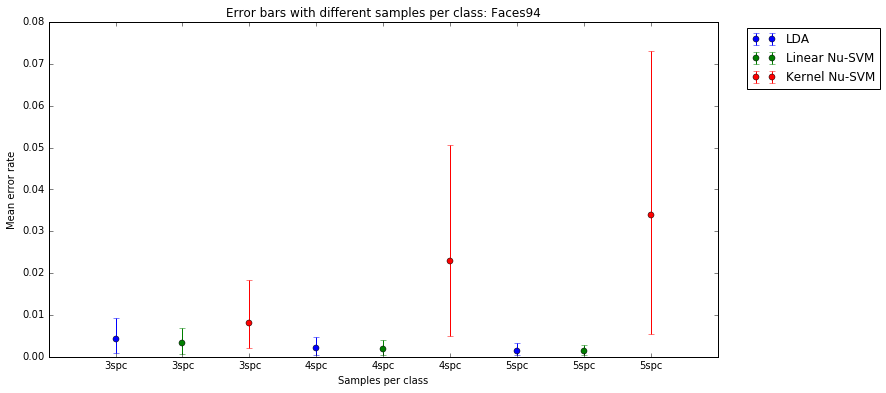
\includegraphics[width=10cm]{ksvm_rescomp94}
\caption{Comparación de resultados obtenidos con RBF SVM en \textbf{Faces94}}
\end{figure}
\end{frame}

\begin{frame}{Resultados RBF SVM Faces95}
\begin{figure}[htpb!]
\centering
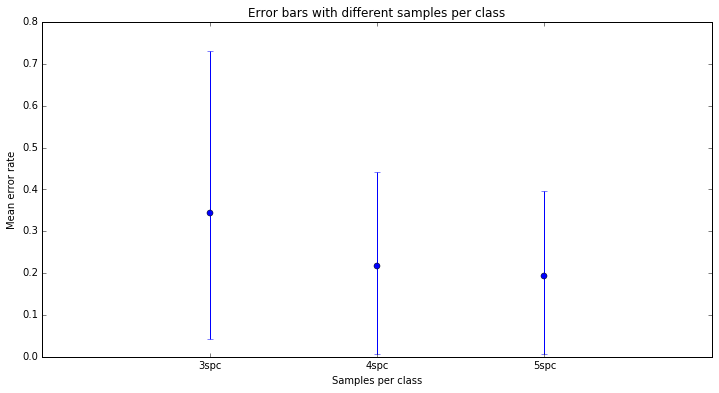
\includegraphics[width=10cm]{ksvm_res95}
\caption{Resultados obtenidos con RBF SVM en \textbf{Faces95}}
\end{figure}
\end{frame}

\begin{frame}{Resultados RBF SVM Faces95 (2)}
\begin{figure}[htpb!]
\centering
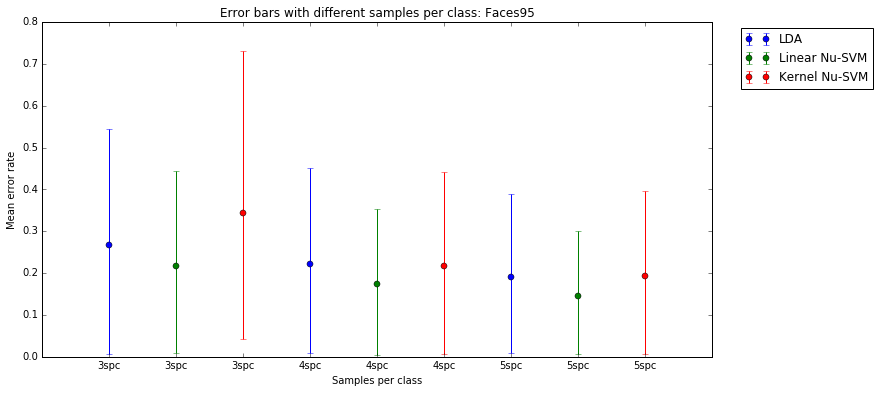
\includegraphics[width=10cm]{ksvm_rescomp95}
\caption{Comparación de resultados obtenidos con RBF SVM en \textbf{Faces95}}
\end{figure}
\end{frame}

\begin{frame}{Análisis de resultados}
\begin{itemize}
	\item Linear-SVM tiene un buen resultado en general, superando a LDA (mejor capacidad de generalización).
	\item Para faces94, ocupar modelos que aumenten la complejidad (como RBF SVM) sólo empeora los resultados. 
	\item Para faces95 RBF SVM se comporta mejor, pero no supera a los otros dos algoritmos anteriores.
\end{itemize}
\end{frame}

\subsection{Convolutional Neural Networks}

\begin{frame}{CNN}
:-(...
\end{frame}




\subsection{Dissimilarity SVM}

\begin{frame}{D-SVM}
\begin{itemize}
	\item Hasta ahora, todos los método tratados resuelven el problema de identificación con clasificación como
	$K$-class clasification.
	\item El método aquí propuesto, transformar el espacio de representación de los datos, reduciendo el problema
	a clasificación binaria.
	\item Para se debe mapear los datos desde el \textit{Image Space} al \textit{Difference Space}. 
	\item Se definen entonces dos conjuntos, $C_1$ y $C_2$; El primero corresponde al \textit{within-class differences set} y contiene las disimilitudes entre datos de la misma clase. El segundo es \textit{between-class difference set} y contiene las disimilitudes entre datos de distinta clase.   
\end{itemize}
\end{frame}


\begin{frame}{D-SVM (2)}
\begin{definition}
 Dea $S_{tr} = \{\mathbf{s}_1 , \ldots, \mathbf{s}_M \}$ el conjunto de entrenamiento con $K$ individuos. Para indicar que dos individuos pertenecen a la misma clase se denota $\mathbf{s}_i \sim \mathbf{s}_j$, y en caso contrario $\mathbf{s}_i \nsim \mathbf{s}_j$. Se define adicionalmente la función de disimilitud $\phi : R^N \times R^N \rightarrow R^S$ con $S \leq N$, como aquella función que mapea dos images, hacia el \textit{difference space}. Luego es posible definir
\begin{align}
& C_1 = \{\phi(\mathbf{s}_i, \mathbf{s}_j)\  | \ \mathbf{s}_i \sim \mathbf{s}_j \} \\
& C_2 = \{\phi(\mathbf{s}_i, \mathbf{s}_j)\  | \ \mathbf{s}_i \nsim \mathbf{s}_j \}
\end{align}
\end{definition}
\end{frame}

\begin{frame}{D-SVM (2)}
\begin{itemize}
	\item El entrenamiento de la D-SVM (Dissimilarity SVM), tiene como entradas los conjuntos $C_1$ y $C_2$.
	\item Como resultado de la clasificación se obtiene la superficie de decisión 
$$
f(\mathbf{x}) = \sum_m^{M_s} \alpha_m y_m K(\mathbf{v}_m, \mathbf{x}) + b = 0
$$
	donde la función $f(\mathbf{x})$ puede ocuparse de discriminante para determinar si un dato pertenece a una clase u a otra.
\end{itemize}
\end{frame}
	
\begin{frame}{D-SVM (3)}
	El proceso de identificación es como sigue
\begin{itemize}
	\item Se $\mathbf{p}$ la imagen a identificar, sobre un conjunto de imagenes conocidas $S_{tr}$ computar la 
	representación en el \textit{difference space}: $\phi(\mathbf{p},\mathbf{s_i}) \ \forall \mathbf{s_i} \in S_{tr}$.
	\item Evaluar la función de discriminante $f(\mathbf{x})$ sobre cada uno de los resultados anteriores.
	\item La clase de pertenencia será aquella para la cual $f(\phi(\mathbf{p},\mathbf{s_i}))$ sea lo menor posible.
\end{itemize}
	
\end{frame}

\begin{frame}{Local Binary Pattern (1)}
\begin{itemize}
	\item \textbf{Idea:} Forma de representación de imágenes, como una composición de micro-patrones que describen
	las estructuras presentes en estas. Los distintos patrones que emergen corresponden a las características presentes
	en las imágenes.
\begin{figure}[htpb!]
\centering
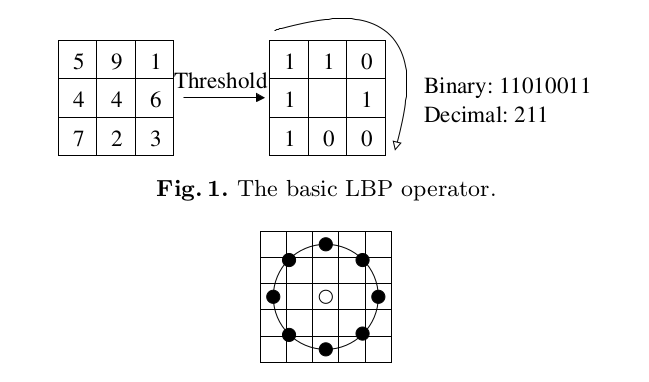
\includegraphics[width=6cm]{lbp}
\caption{Local Binary Pattern Operator}
\end{figure}
\end{itemize}
\end{frame}

\begin{frame}{Local Binary Pattern (2)}
\begin{figure}[htpb!]
\centering
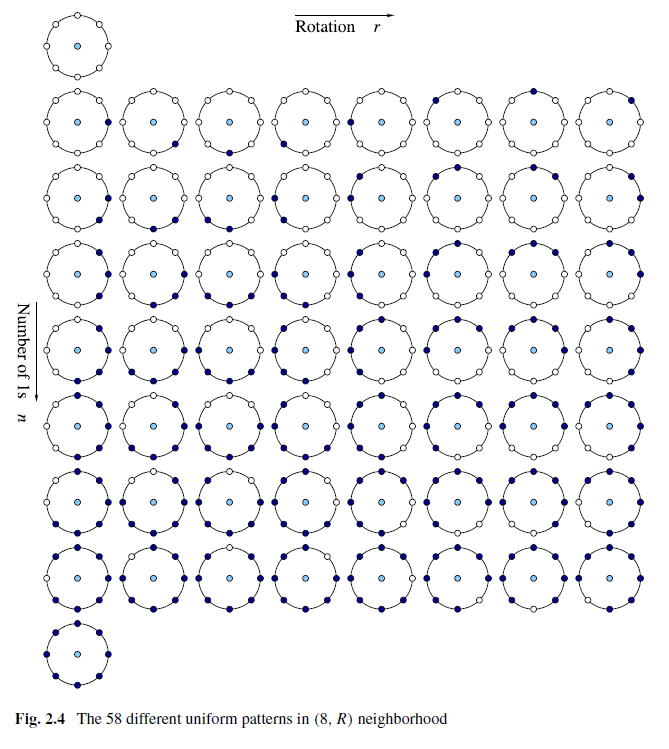
\includegraphics[width=5cm]{uniform_lbp}
\caption{Uniform Local Binary Patterns}
\end{figure}
\end{frame}



\begin{frame}{Histograma Espacial de Características}
\begin{itemize}
	\item Cada uno de estos 59 patrones representan una característica, y la frecuencia o distribución (histogramas) de estas define las estructuras presentes en las imagenes.
	\item Sin embargo se requiere también de información espacial, acerca de donde se encuentran estas características.
\begin{figure}[htpb!]
\centering
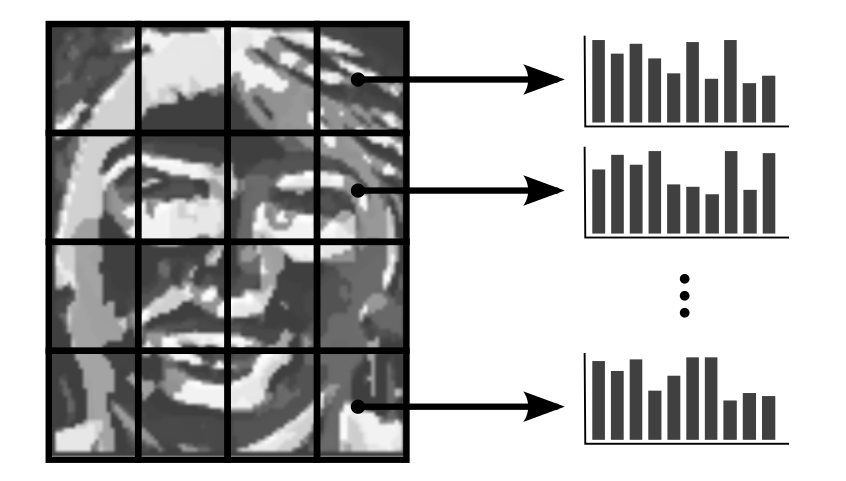
\includegraphics[width=5cm]{spatial_hist}
\caption{Histograma espacial de características}
\end{figure}
\end{itemize}
\end{frame}


\begin{frame}{Método Propuesto}
El modelo propuesto difiere de aquel propuesto por P. Jonathon Philips en \textit{Support Vector Machines Applied to Face Recognition}, en la función $\phi(\cdot,\cdot)$ de mapeo al \textit{difference space}. Sean dos imagenes representadas en la forma de histograma espacial $(\mathbf{h_1},\mathbf{h_2})$ con $S$ histogramas, luego la función es

\begin{definition}
	$\phi(\mathbf{h_1}, \mathbf{h_2}) = \mathbf{d} = (d_1, \cdots, d_S)$ tal que $\mathbf{d_i}$ corresponde a la diferencia existente entre los histogramas $i$-ésimos de las respectivas imágenes. Tal diferencia se computa con la función:
	$$\chi^2(x,y) = \sum_k \frac{(x_k - y_k)^2}{x_K + y_k}$$
\end{definition}
\end{frame}


\begin{frame}{Detalles de Implementación}
\begin{itemize}
	\item Cuando existen $s$ muestras por clase, se pueden hacer $\binom{s}{2}$ combinaciones para formar el conjunto $C_1$.
	\item El conjunto $C_2$ se forma tomando aleatoreamente igual cantidad ($\binom{s}{2}$) de pares de datos de distinta clase.
	\item El valor que obtiene la función discriminante $f(\mathbf{x})$, se promedia para los datos que pertenecen a la misma clase en $S_{tr}$
\end{itemize}
\end{frame}


\begin{frame}{Resultados D-SVM Faces94}
\begin{figure}[htpb!]
\centering
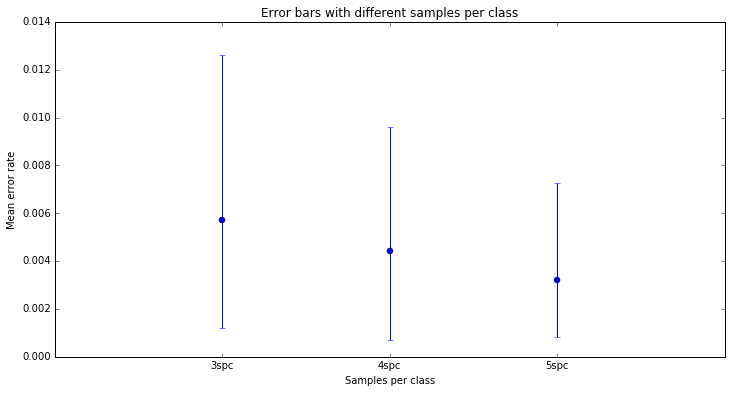
\includegraphics[width=10cm]{dsvm_res94}
\caption{Resultados obtenidos con D-SVM en \textbf{Faces94}}
\end{figure}
\end{frame}

\begin{frame}{Resultados D-SVM Faces94 (2)}
\begin{figure}[htpb!]
\centering
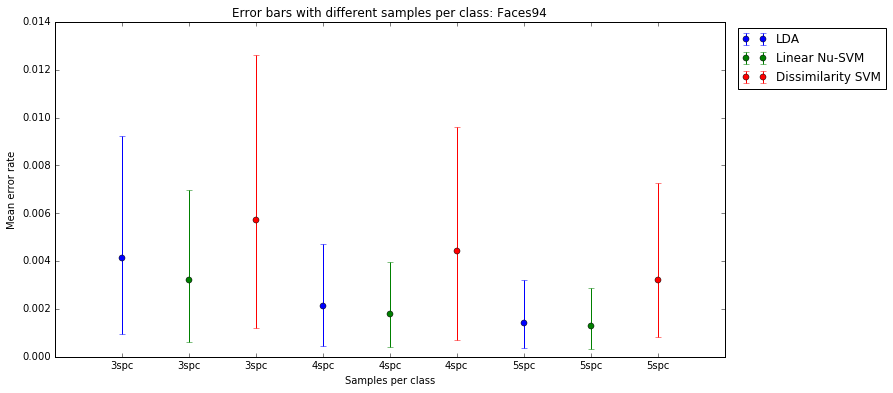
\includegraphics[width=10cm]{dsvm_rescomp94}
\caption{Comparación de resultados obtenidos con D-SVM en \textbf{Faces94}}
\end{figure}
\end{frame}

\begin{frame}{Resultados D-SVM Faces95}
\begin{figure}[htpb!]
\centering
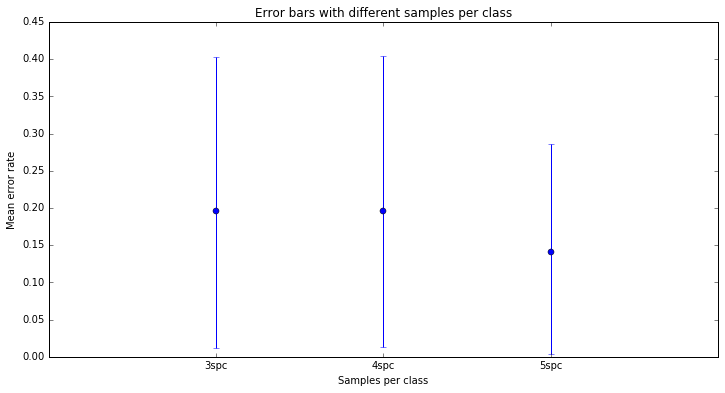
\includegraphics[width=10cm]{dsvm_res95}
\caption{Resultados obtenidos con D-SVM en \textbf{Faces95}}
\end{figure}
\end{frame}

\begin{frame}{Resultados D-SVM Faces95 (2)}
\begin{figure}[htpb!]
\centering
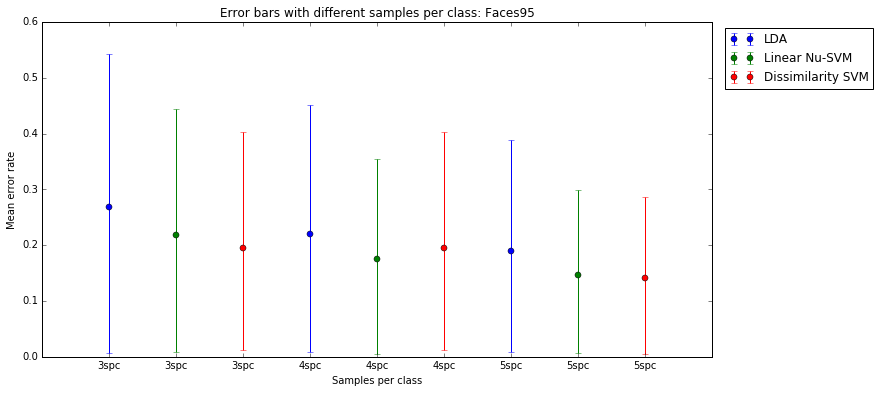
\includegraphics[width=10cm]{dsvm_rescomp95}
\caption{Comparación de resultados obtenidos con D-SVM en \textbf{Faces95}}
\end{figure}
\end{frame}




% All of the following is optional and typically not needed.
% \appendix
% \section<presentation>*{\appendixname}
% \subsection<presentation>*{For Further Reading}

% \begin{frame}[allowframebreaks]
%   \frametitle<presentation>{For Further Reading}
    
%   \begin{thebibliography}{10}
    
%   \beamertemplatebookbibitems
%   % Start with overview books.

%   \bibitem{Author1990}
%     A.~Author.
%     \newblock {\em Handbook of Everything}.
%     \newblock Some Press, 1990.
 
    
%   \beamertemplatearticlebibitems
%   % Followed by interesting articles. Keep the list short.

%   \bibitem{Someone2000}
%     S.~Someone.
%     \newblock On this and that.
%     \newblock {\em Journal of This and That}, 2(1):50--100,
%     2000.
%   \end{thebibliography}
% \end{frame}

\end{document}